\appendix
\chapter*{LAMPIRAN}
\addcontentsline{toc}{chapter}{LAMPIRAN}
\setcounter{section}{0} % Mengatur ulang penomoran section
\setcounter{page}{1}

\renewcommand{\thesection}{\Alph{section}}
\renewcommand{\thesubsection}{\Alph{section}.\arabic{subsection}\hspace{-0.25cm}}
\renewcommand{\thepage}{L - \arabic{page}}


%1. Surat Tugas Pelaksanaan KP
%
%2. Surat Balasan dari Perusahaan (bukti diterima PI)
%
%3. Logbook Kegiatan Praktik Industri
%
%4. Daftar Hadir
%
%5. Form Nilai dari Industri, format klik di sini
%
%6. Dokumentasi Kegiatan (Foto-foto)


\numberwithin{figure}{section}
\section{Surat Balasan dari Perusahaan (bukti diterima PI)}
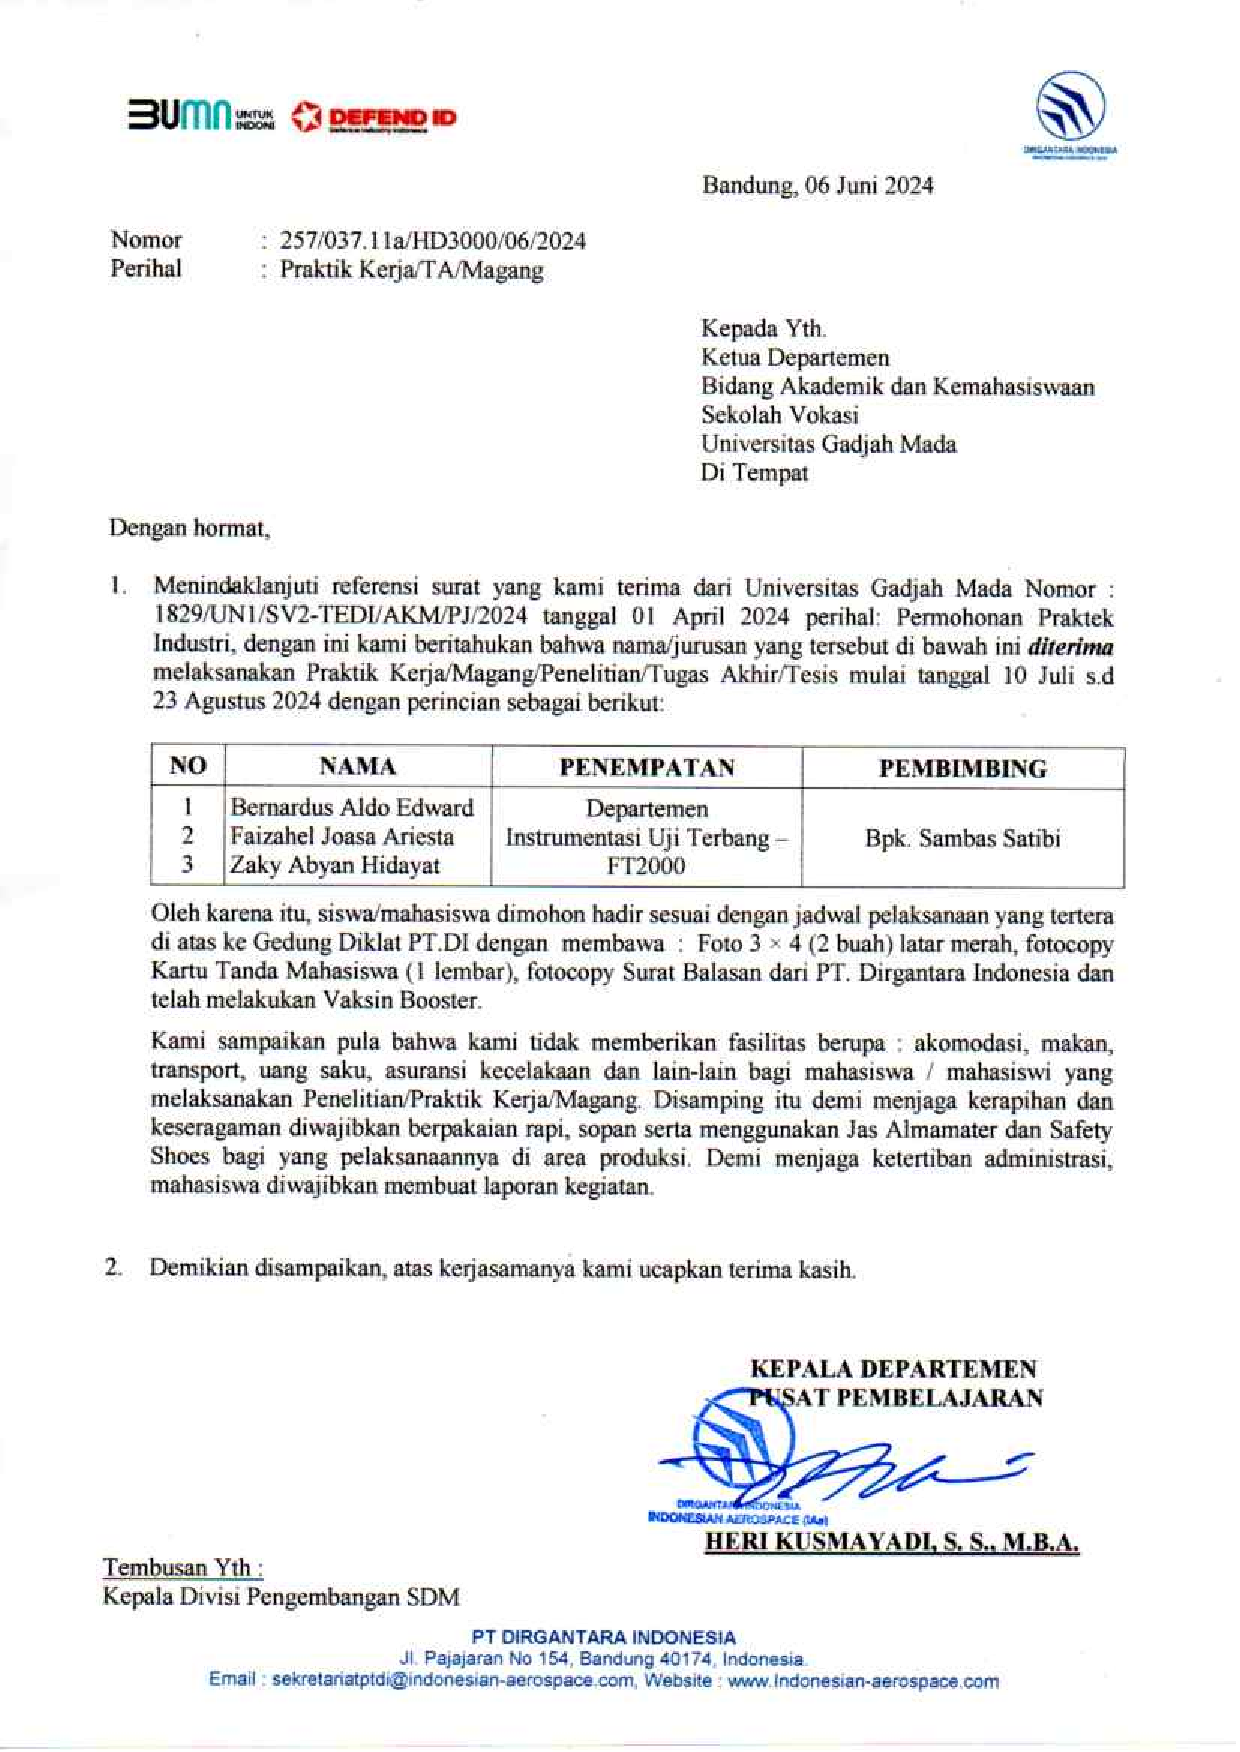
\includegraphics[scale=0.7]{dokumen/magang-ptdi.pdf}

\newpage
\section{Surat Tugas Praktik Industri}
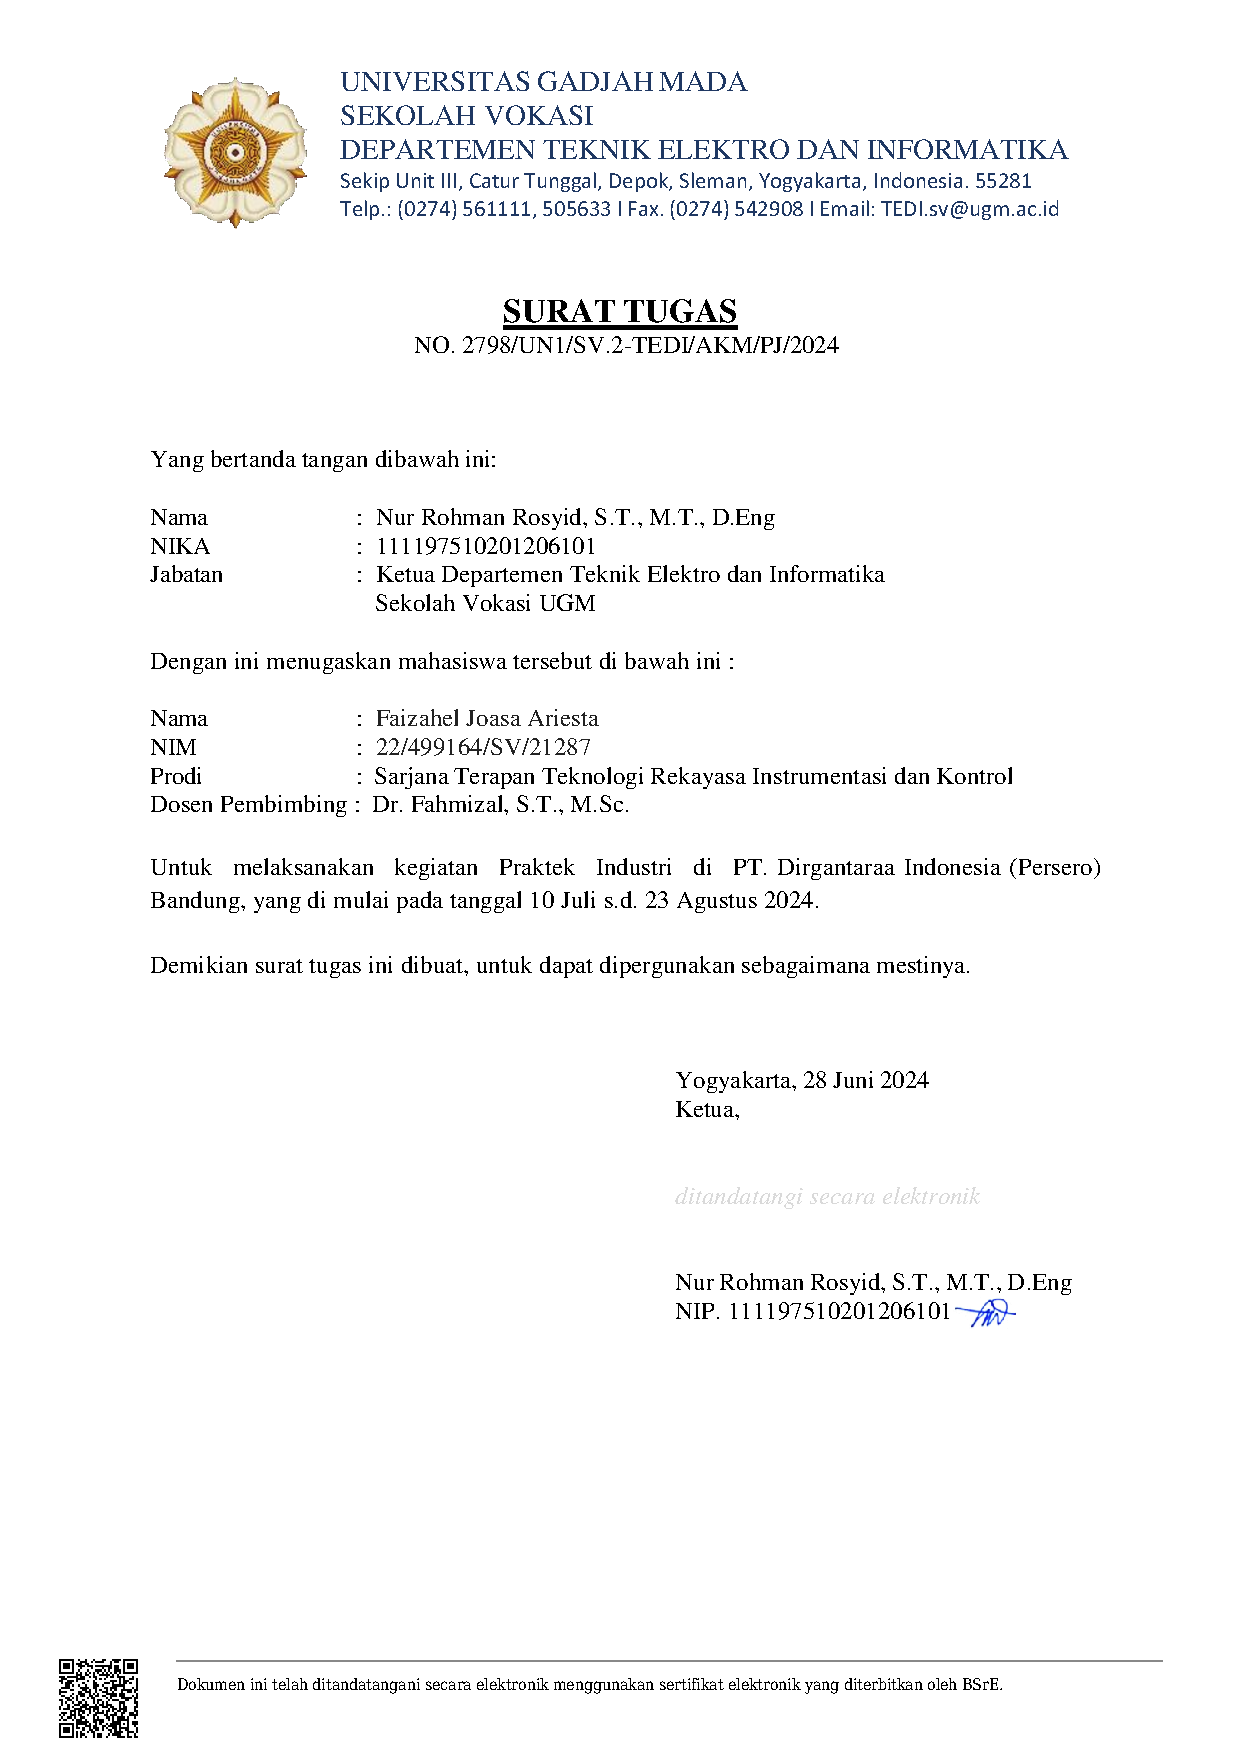
\includegraphics[scale=0.7]{dokumen/suratTugas.pdf}

\newpage
\section{Logbook Kegiatan Praktik Industri}
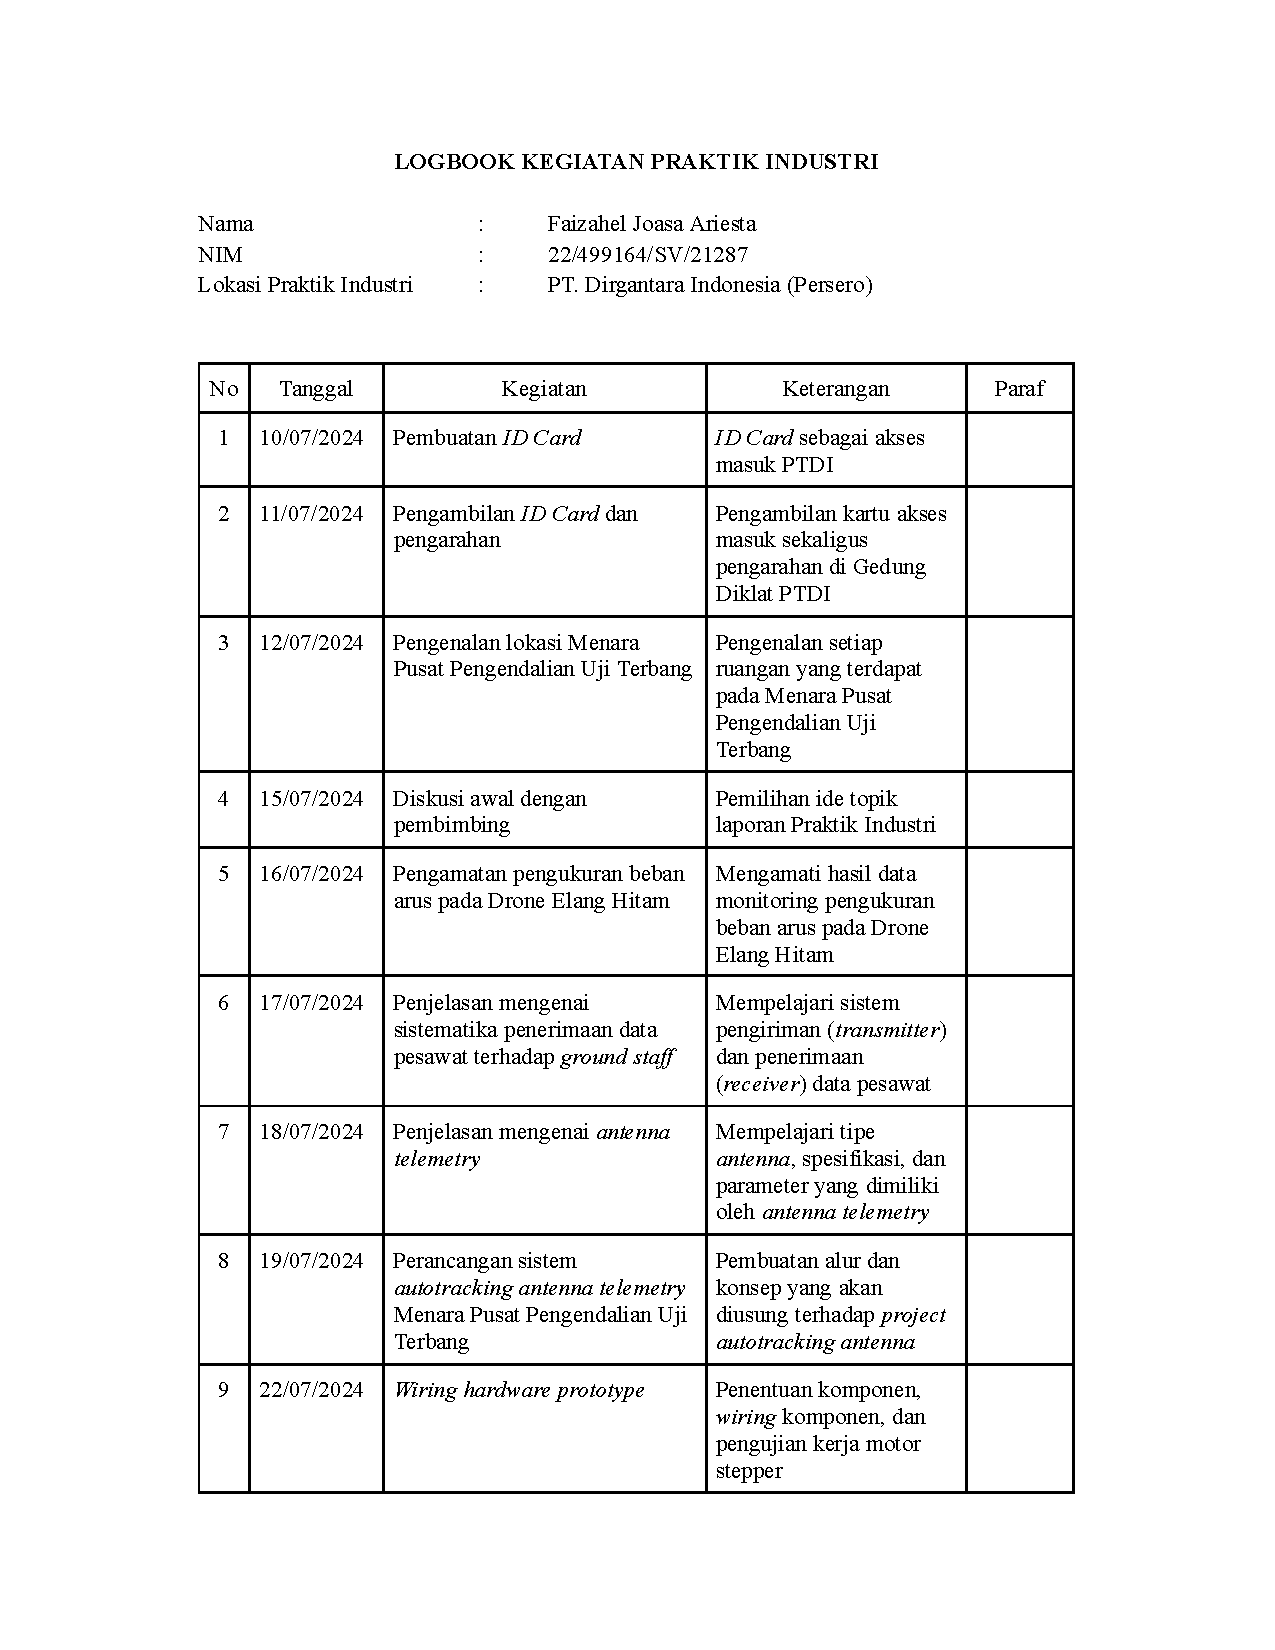
\includegraphics[scale=0.7,page=1]{dokumen/logbook.pdf}
\newpage
\includegraphics[scale=0.7,page=2]{dokumen/logbook.pdf}
\newpage
\includegraphics[scale=0.7,page=3]{dokumen/logbook.pdf}
\newpage
\includegraphics[scale=0.7,page=4]{dokumen/logbook.pdf}

\newpage
\section{Daftar Hadir Praktik Industri}
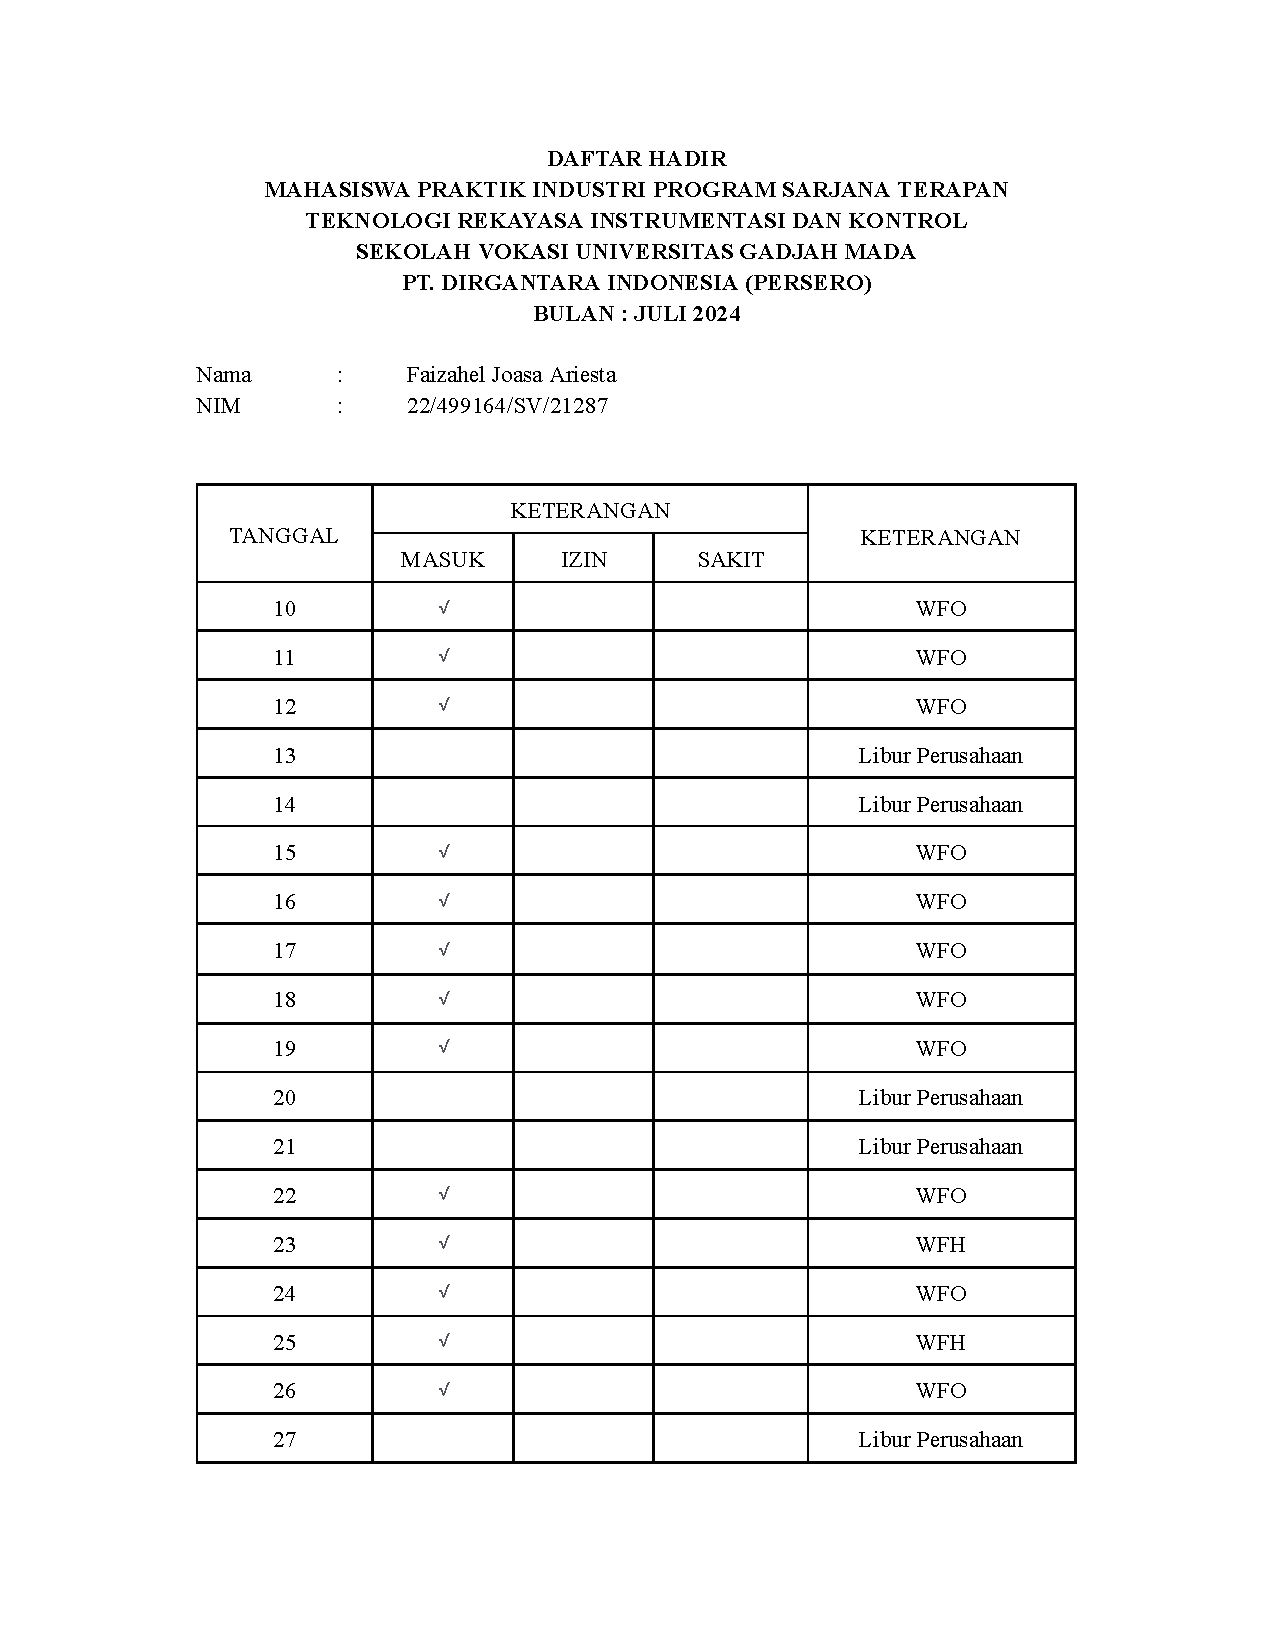
\includegraphics[scale=0.7,page=1]{dokumen/daftarhadir.pdf}
\newpage
\includegraphics[scale=0.7,page=2]{dokumen/daftarhadir.pdf}
\newpage
\includegraphics[scale=0.7,page=3]{dokumen/daftarhadir.pdf}
\newpage
\includegraphics[scale=0.7,page=4]{dokumen/daftarhadir.pdf}


\newpage
\section{Penilaian Hasil Kegiatan Praktik Industri}
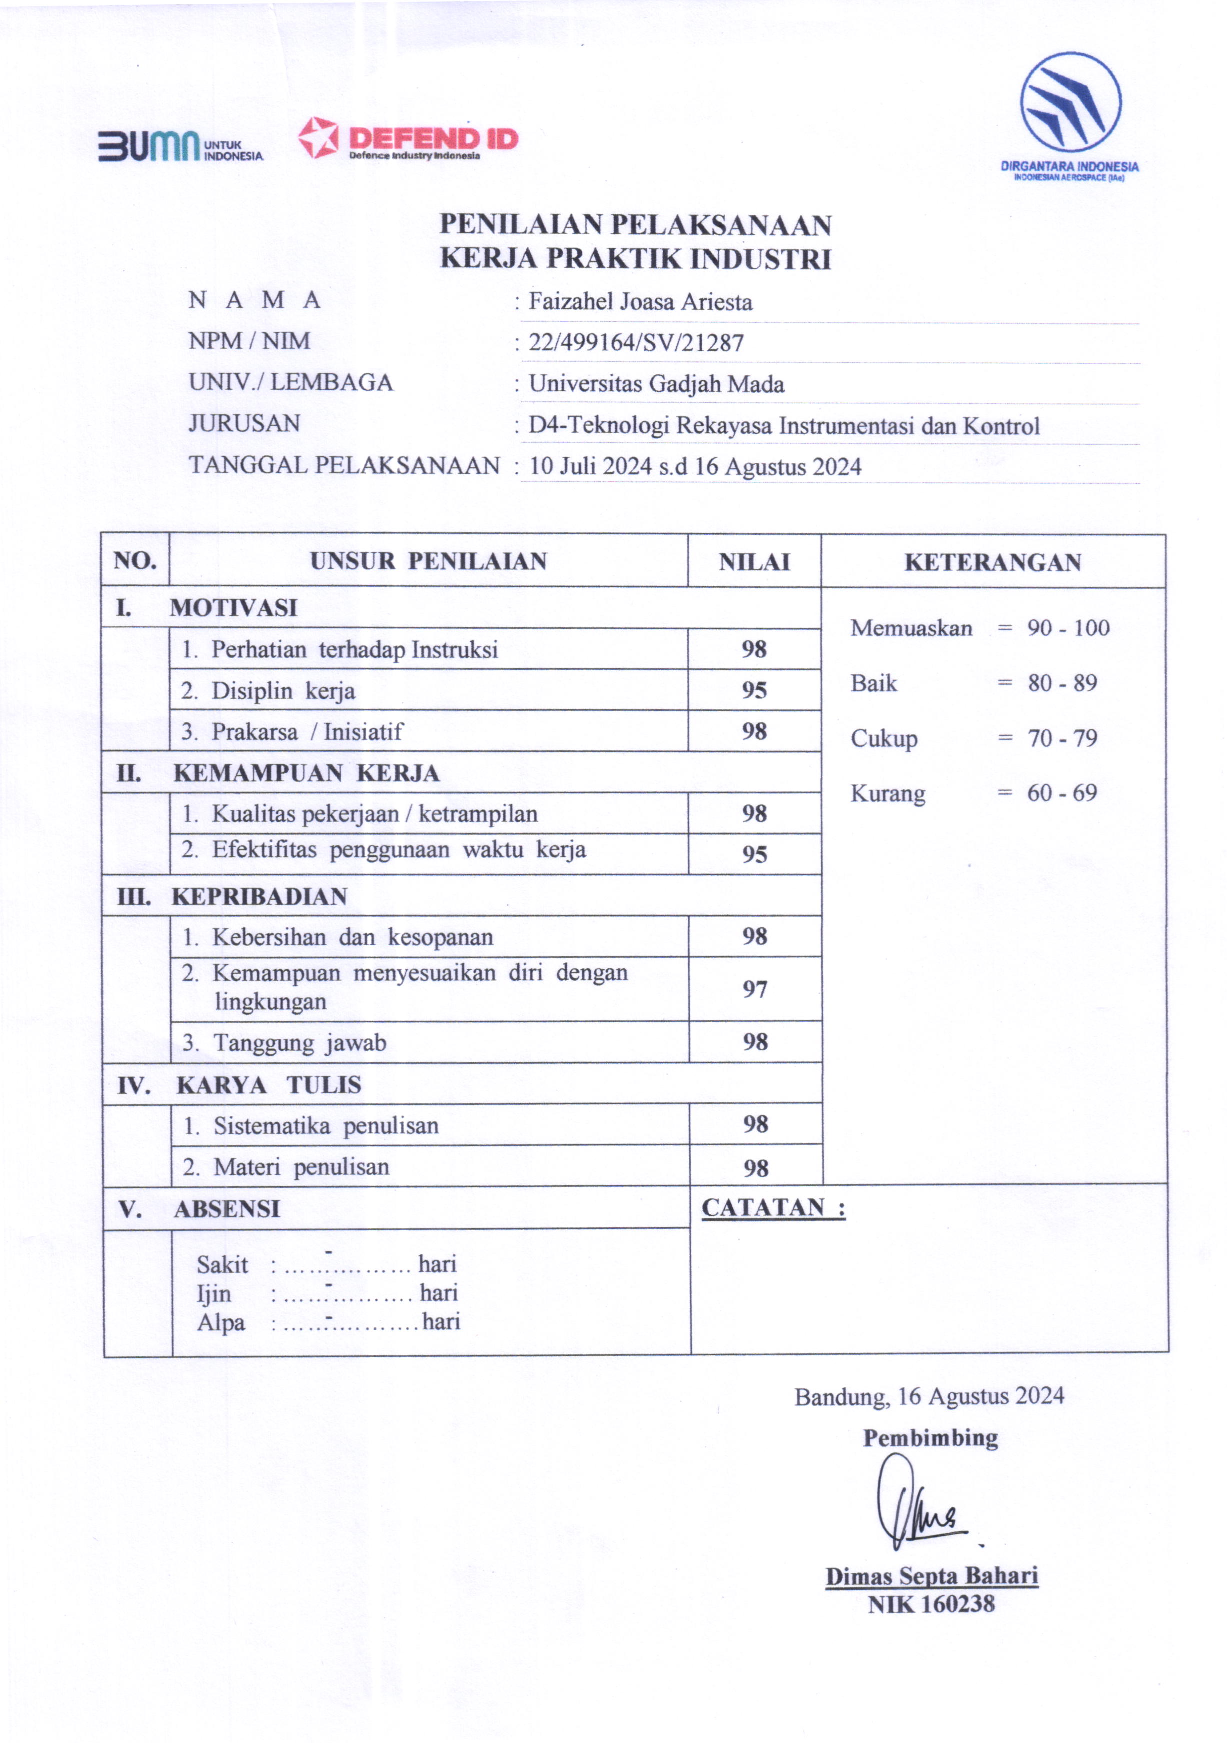
\includegraphics[scale=0.7]{dokumen/nilai-perusahaan.pdf}

\newpage
\section{Surat Keterangan Selesai Praktik Industri}
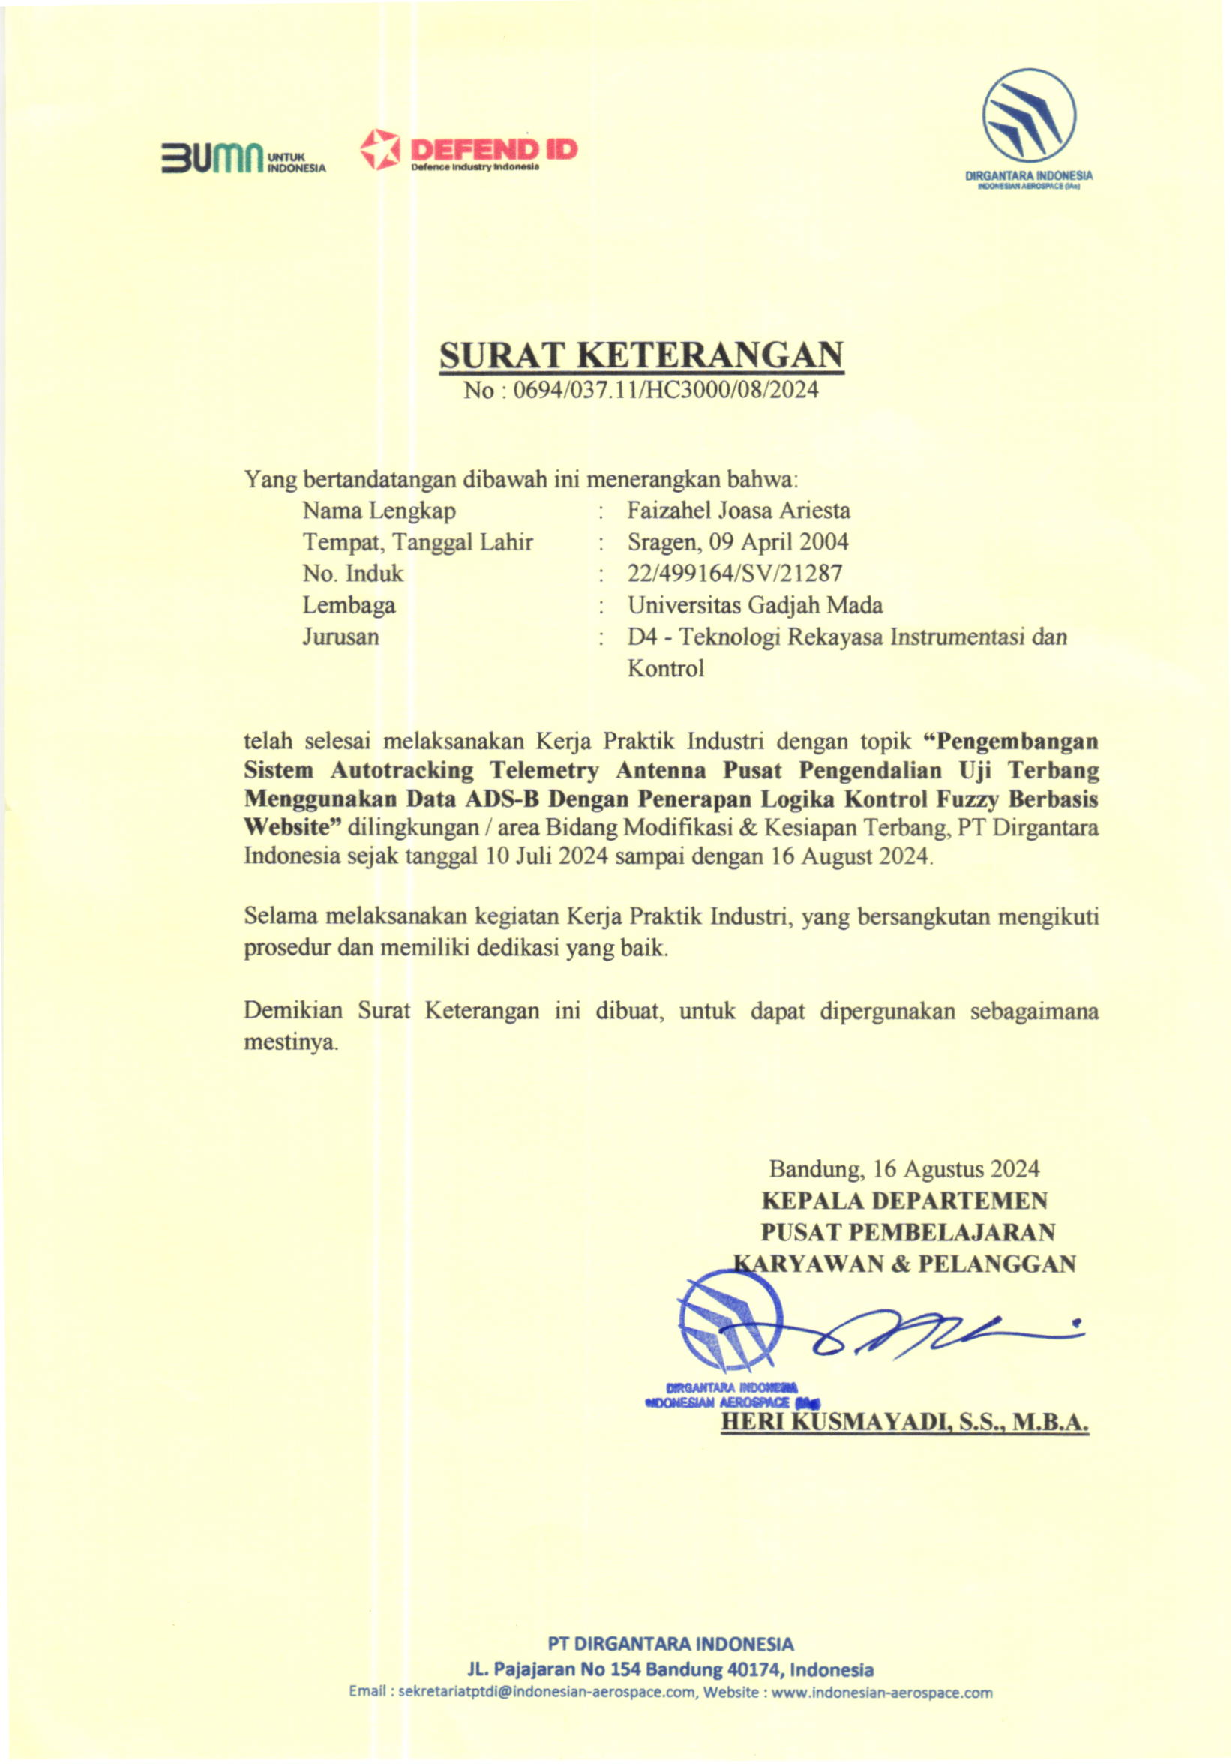
\includegraphics[scale=0.7]{dokumen/pernyataanSelesai.pdf}

\newpage
\section{Dokumentasi}
\begin{figure}[H]
	\centering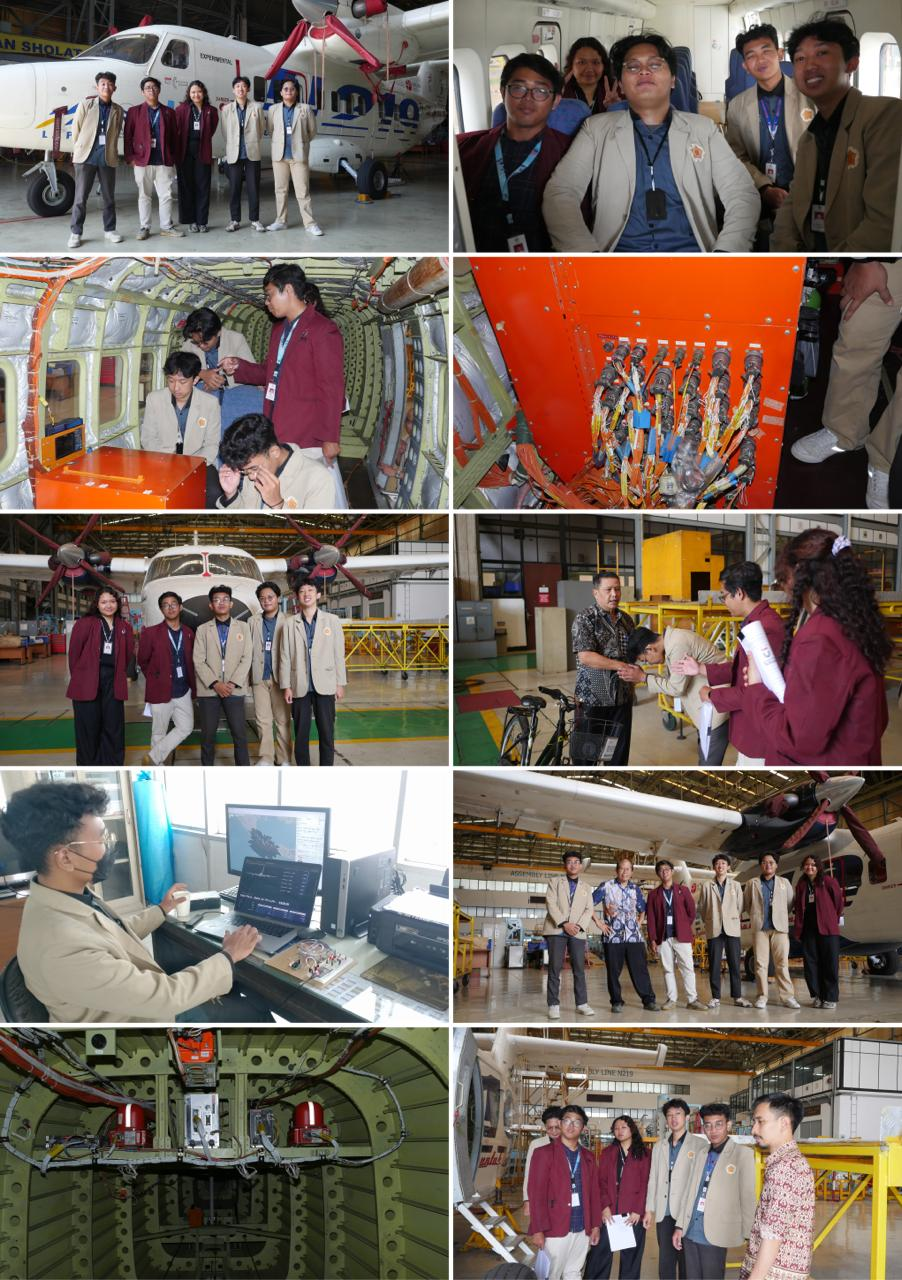
\includegraphics[width = 0.9\textwidth]{gambar/dokumentasi.jpeg}
	\caption{Dokumentasi Kegiatan Praktik Industri di PT Dirgantara Indonesia (Persero)}
\end{figure}




